Los resultados de cierto experimento relacionan las variables $x$ e $y$, mediante el modelo:
$$
y=\beta x^{\alpha x}.
$$
Estos resultados se muestran en la siguiente tabla:
\begin{center}
\begin{tabular}{c|ccccc}
$x$ & 1 & 1.5 & 2 & 3 & 4\\
\hline
$y$ & 85 & 60 & 15 & 3 & 1
\end{tabular}
\end{center}
Escriba un rutero en \matlab que realice las siguientes tareas:
\begin{enumerate}
\item Proponga una transformaci\'on que linealice el modelo

\respuesta{4cm}

\item Calcule y muestre los par\'ametros $\alpha$ y $\beta$ que ajustan el modelo a los datos de la tabla en el sentido de los m\'inimos cuadrados.
\item En un mismo gr\'afico dibuje los puntos de la tabla (c\'irculos) y el modelo ajustado anteriormente (linea continua).
\item Estime y muestre el valor de $y$ cuando $x=5$.
\end{enumerate}

\textbf{Desarrollo:} El rutero est\'a dado por:

Se observa que mediante una funci\'on logaritmo
$$
y=\beta x^{\alpha x} \leftrightarrow ln(y) =ln(\beta)+ \alpha x ln(x)
$$
\hfill\fbox{10pt}

con lo cual se hace un programa parecido a
\begin{lstlisting}
x=[1 1.5 2 3 4]';
y=[85 60 15 3 1]';
A = [ones(5,1) x.*log(x)];
B = log(y);
X = A\B					%15 PUNTOS
alpha = X(2);
beta = exp(X(1));
xx = 1:0.01:4;
yy = beta*xx.^(alpha*xx);
plot(x,y,'o',xx,yy,'-')
legend('Datos','Modelo') 	%10 PUNTOS
x5=5;
y5 = beta*x5.^(alpha*x5) 	%5 PUNTOS
\end{lstlisting}

mientras que el gr\'afico est\'a dado por:

\centerline{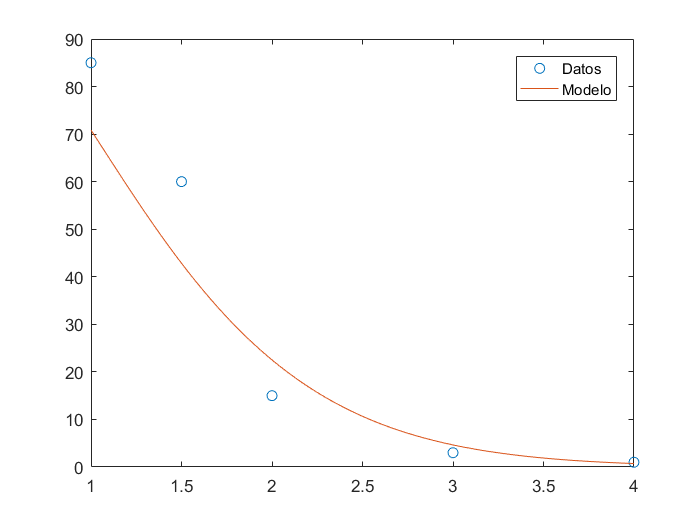
\includegraphics[width=0.6\textwidth]{mincuad.png}}
